\section{1174077 - Alvan Alvanzah}
\subsection{Soal Teori}
\begin{enumerate}

	\item Jelaskan kenapa file teks harus di lakukan tokenizer
	\hfill\break
    Jelaskan kenapa file teks harus di lakukan tokenizer. dilengkapi dengan ilustrasi atau gambar. 
    \hfill \break
    Tokenizer diperlukan untuk perhitungan bobot pada setiap teks karena Tokenizer akan membagi kalimat menjadi beberapa teks sehingga nantinya kalimat yang dimasukkan otomatis langsung diubah menjadi kata - kata dan akan dinilai sehingga akan memunculkan nilai vektor untuk digunakan saat prediksi teks yang muncul pada satu kalimat tersebut. Biasanya untuk memisahkan sebuah kata, tokenizer akan menggunakan spasi sebagai pemisah antar kata.
    
    \begin{figure}[H]
	\centering
		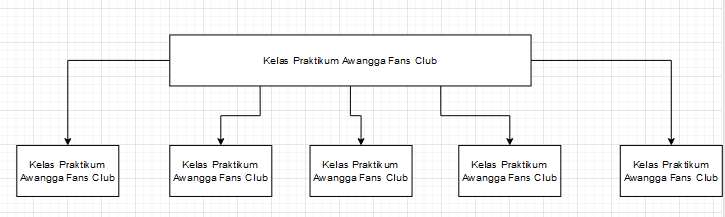
\includegraphics[width=4cm]{figures/1174077/7/teori_1.PNG}
		\caption{Ilustrasi Tokenizer}
	\end{figure}

	\item Jelaskan konsep dasar K Fold Cross Validation pada dataset komentar Youtube pada kode listing 7.1 \ref{lst:7.0}
    \begin{lstlisting}[caption=K Fold Cross Validation,label={lst:7.0}]
        kfold = StratifiedKFold(n_splits=5)
        splits = kfold.split(d, d['CLASS'])
        \end{lstlisting}
    \hfill\break
    Pada koding diatas terdapat variabel kfold yang didalamnya berisi parameter split yang diisikan nilai 5. hal tersebut dimaksudkan untuk membuat pengolahan data akan diulang setiap datanya sebanyak lima kali dengan atribut class sebagai acuan pengolahan datanya. Lalu kemudian akan di hasilkan akurasi dari pengulangan data tersebut sebesar sekian persen tergantung datanya	
    \begin{figure}[H]
	\centering
		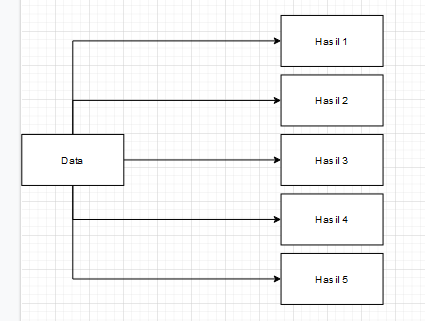
\includegraphics[width=4cm]{figures/1174077/7/teori_2.PNG}
		\caption{ilustrasi K-Fold Cross Validation}
	\end{figure}

	\item Jelaskan apa maksudnya kode program for train, test in splits.
	\hfill\break
	For train digunakan untuk melakukan training atau pelatihan pada data yang sudah dideklarasikan sebelumnya. Sedangkan test in split digunakan untuk membatasi jumlah data yang akan diinputkan atau data yang akan digunakan.
    \begin{figure}[H]
        \centering
            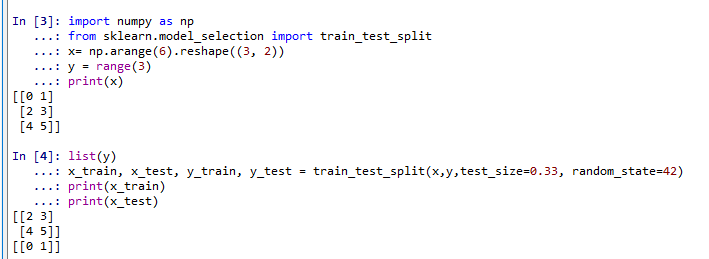
\includegraphics[width=4cm]{figures/1174077/7/teori_3.PNG}
            \caption{Ilustrasi for train dan test in split}
        \end{figure}

	\item Jelaskan apa maksudnya kode program train content = d[’CONTENT’].iloc[train idx] dan test content = d[’CONTENT’].iloc[test idx].
	\hfill\break
	Maksud dari kode program tersebut adalah membaca isian kolom pada field yang bernama CONTENT sebagai data training dan data testing untuk program 
    \begin{figure}[H]
	\centering
		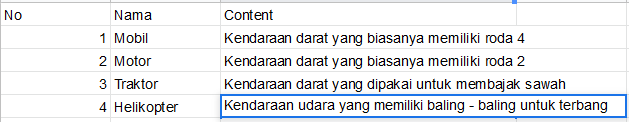
\includegraphics[width=4cm]{figures/1174077/7/teori_4.PNG}
		\caption{ilustrasi penggunaan kolom content}
	\end{figure}

	\item Jelaskan apa maksud dari fungsi tokenizer = Tokenizer(num words=2000) dan tokenizer.fit on texts(train content).
	\hfill\break
	\begin{itemize}
        \item tokenizer = Tokennizer(num\_words=2000) digunakan untuk membaca kalimat yang telah dibuat menjadi token sebanyak 2000 kata
        \item fit\_on\_texts digunakan untuk membuat membaca data token teks yang telah dimasukan kedalam fungsi yaitu fungsi train\_konten
    \end{itemize}
	\begin{figure}[H]
	\centering
		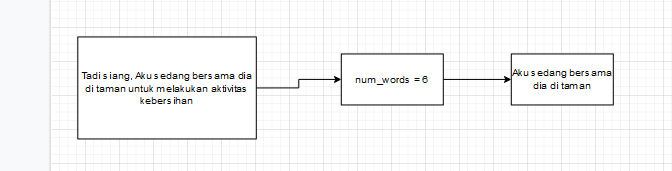
\includegraphics[width=4cm]{figures/1174077/7/teori_5.PNG}
		\caption{Ilustrasi Fit Tokenizer dan num\_word=2000}
	\end{figure}

	\item Jelaskan apa maksud dari fungsi d train inputs = tokenizer.texts to matrix(train content, mode=’tfidf’) dan d test inputs = tokenizer.texts to matrix(test content, mode=’tfidf’), 
	\hfill\break
	Untuk digunakan sebagai pengubah urutan teks yang tadi telah dilakukan tkoenizer menjadi matriks yang berurutan seperti tf idf
	\begin{figure}[H]
	    \centering
	    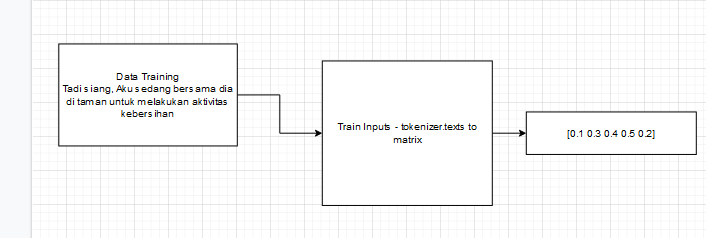
\includegraphics[width=4cm]{figures/1174077/7/teori_6.PNG}
	    \caption{Ilustrasi d train inputs = tokenizer.texts to matrix}
    \end{figure}

    \item  Jelaskan apa maksud dari fungsi d train inputs = d train inputs/np.amax(np.absolute(d train dan d test inputs = d test inputs/np.amax(np.absolute(d test inputs))
    \hfill\break
    Fungsi tersebut digunakan untuk membagi matriks tfidf dnegan penentuan maksimum array sepanjang sumbu sehingga akan menimbulkan garis ke bawah dan ke atas yang membentuk gambar v. Lalu hasil tersebut akan dimasukkan ke variabel d train input dan d test input dengan methode absolute. Yang berarti tanpa bilangan negatif.
    \begin{figure}[H]
	    \centering
	    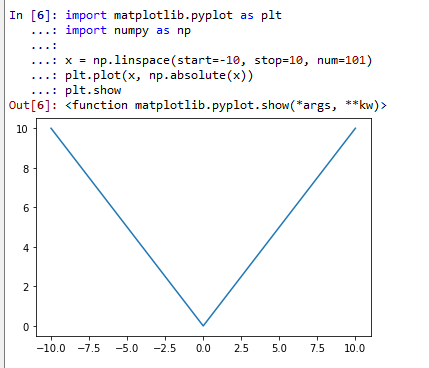
\includegraphics[width=4cm]{figures/1174077/7/teori_7.PNG}
	    \caption{fungsi d train inputs}
    \end{figure}

    \item Jelaskan apa maksud fungsi dari d train outputs = np utils.to categorical(d[’CLASS’].iloc[train dan d test outputs = np utils.to categorical(d[’CLASS’].iloc[test idx]) dalam kode program
    \hfill\break
    Maksud dari fungsi tersebut yaitu untuk merubah nilai vektor yang ada pada atribut class menjadi bentuk matrix dengan pengurutan berdasarkan data index training dan testing.
    \begin{figure}[H]
	    \centering
	    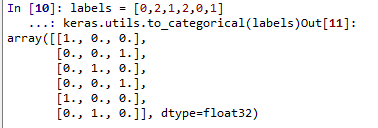
\includegraphics[width=4cm]{figures/1174077/7/teori_8.PNG}
	    \caption{fungsi train outputs = np utils.to categorical}
    \end{figure}

    \item Jelaskan apa maksud dari fungsi di listing 7.2 \ref{lst:7.1}. 
    \begin{lstlisting}[caption=Membuat model Neural Network,label={lst:7.1}]
        model = Sequential()
        model.add(Dense(512, input_shape=(2000,)))
        model.add(Activation('relu'))
        model.add(Dropout(0.5))
        model.add(Dense(2))
        model.add(Activation('softmax'))
    \end{lstlisting}
    \hfill\break
    model = sequential berarti variabel model berisi method sequential yang berguna untuk searching data dengan menerima parameter atau argumen kunci dengan langkah tertentu untuk mencari data yang telah diolah. Kemudian model akan ditambahkan method add dengan dense yang berarti data - data yang diinputkan akan terhubung, dengan data 612 dan 2000 data kata atau word kemudian model tersebut di masukan fungsi activation dengan rumus atau metode relu. setelah itu data akan di dropout 0.5atau dipangkas sebanyak 50 persen dikarenakan pada pohon bobot terlalu akurat terhadap data.
    \begin{figure}[H]
	    \centering
	    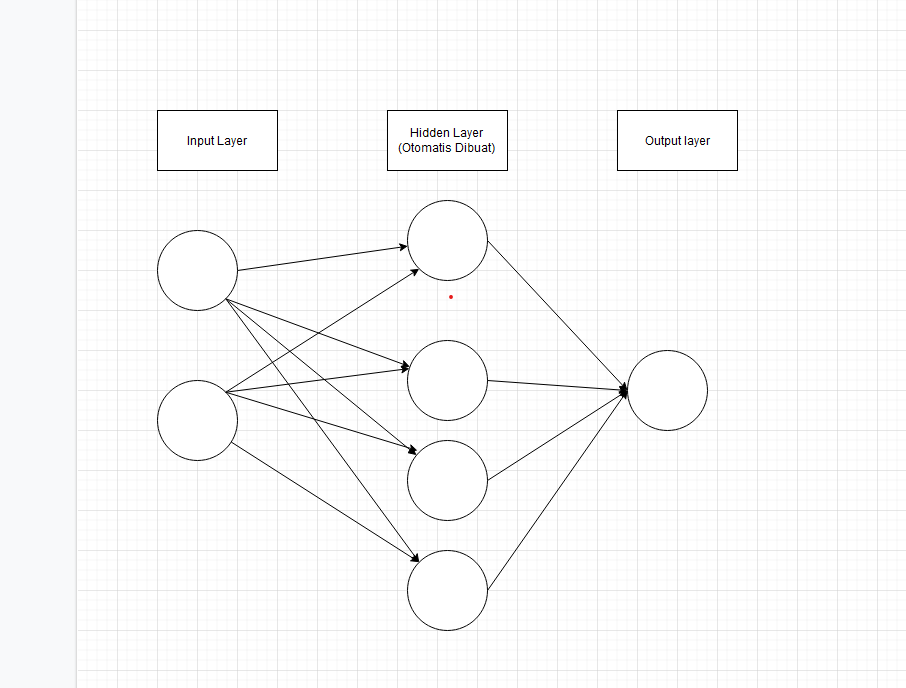
\includegraphics[width=4cm]{figures/1174077/7/teori_9.PNG}
	    \caption{ilustrasi neural network}
    \end{figure}

    \item Jelaskan apa maksud dari fungsi di listing 7.3 \ref{lst:7.2}  dengan parameter tersebut.
    \begin{lstlisting}[caption=Compile model,label={lst:7.2}]
        model.compile(loss='categorical_crossentropy', optimizer='adamax',
                          metrics=['accuracy'])
    \end{lstlisting}
    model tersebut kemudian di compile atau di kembalikan kembali fungsi nilainya yangmana akan mengembalikan fungsi nilai loss nya berapa yang diambil dari fungsi adamax yang berberguna untuk mengetahui nilai lossnya kemudian metrics = acuracy merupakan akurasi dari nilai matrixnya. kemudian terdiri atas beberapa layer atau hiden layer. perbedaan antara deep learning dan DNN atau Deep Neural Network yaitu deep lerning merupakan pemakai algoritma dari DNN dan DNN merupakan algoritma yang ada pada deep learning.

    \item Jelaskan apa itu Deep Learning
    \hfill\break
    Deep learning merupakan salah satu algoritma yang seperti Neural Network yang menggunakan meta data sebagai inputan dan mengolahnya menggunakan layer layer yang tersembunyi.

    \item Jelaskan apa itu Deep Neural Network, dan apa bedanya dengan Deep Learning
    \hfill\break
    Deep Neural Network merupakan algoritma jaringan syaraf yang melakukan pembobotan terhadap data yang sudah ada sebagai acuan untuk data inputan selanjutnya. 

    \item Jelaskan dengan ilustrasi gambar buatan sendiri(langkah per langkah) bagaimana perhitungan algoritma konvolusi dengan ukuran stride (NPM mod3+1) x (NPM mod3+1) yang terdapat max pooling.
    \hfill\break
    Sebelum membuat ilustrasi perlu di ketahui apa itu stride, stride adalah acuan atau parameter yang menentukan pergeseran pada filter fixcel. sebagai contoh nilai stride 1 yang berarti filter akan bergeser sebanyak satu fixcel secara vertikal dan horizontal. selanjutnya apa itu max pooling contoh pada suatu gambar di tentukan Max Pooling dari 3 x 3 dengan stride 1 yang berarti setiap pergeseran 1 pixcel akan diambil nilai terbesar dari pixcel 3 x 3 tersebut.
    \begin{figure}[H]
	    \centering
	    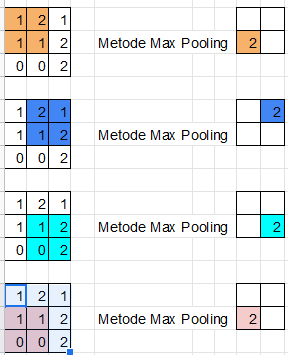
\includegraphics[width=4cm]{figures/1174077/7/teori_10.PNG}
	    \caption{ilustrasi perhitungan stride 1 max pooling}
    \end{figure}
\end{enumerate}

\subsection{Praktek Program}
\begin{enumerate}
	\item  Jelaskan kode program pada blok \# In[1]. Jelaskan arti dari setiap baris kode yang dibuat(harus beda dengan teman sekelas) dan hasil luarannya dari komputer sendiri.
	\hfill\break
	\lstinputlisting[firstline=1, lastline=8]{src/1174077/7/1174077.py}
	\begin{figure}[H]
	\centering
		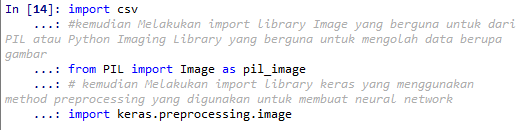
\includegraphics[width=4cm]{figures/1174077/7/praktek_1.PNG}
		\caption{Hasil Soal 1.}
	\end{figure}

	\item  Jelaskan kode program pada blok \# In[2]. Jelaskan arti dari setiap baris kode yang dibuat(harus beda dengan teman sekelas) dan hasil luarannya dari komputer sendiri.
	\hfill\break
	\lstinputlisting[firstline=9, lastline=36]{src/1174077/7/1174077.py}
	\begin{figure}[H]
	\centering
		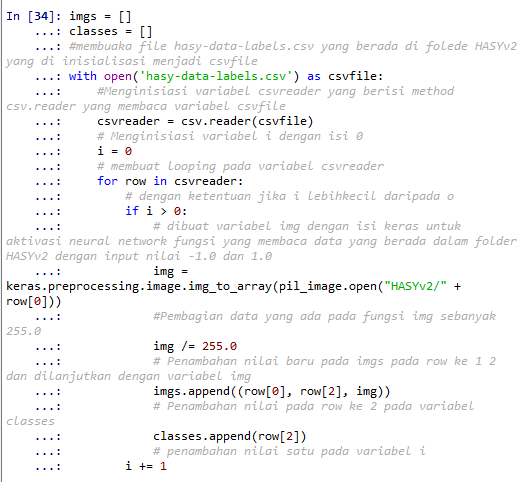
\includegraphics[width=4cm]{figures/1174077/7/praktek_2.PNG}
		\caption{Hasil Soal 2.}
	\end{figure}

	\item Jelaskan kode program pada blok \# In[3]. Jelaskan arti dari setiap baris kode yang dibuat(harus beda dengan teman sekelas) dan hasil luarannya dari komputer sendiri.
	\hfill\break
	\lstinputlisting[firstline=37, lastline=48]{src/1174077/7/1174077.py}
	\begin{figure}[H]
	\centering
		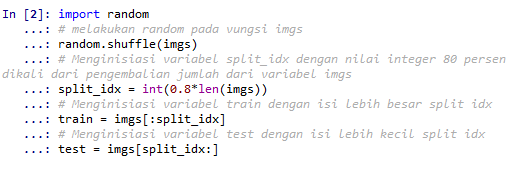
\includegraphics[width=4cm]{figures/1174077/7/praktek_3.PNG}
		\caption{Hasil Soal 3.}
	\end{figure}

	\item Jelaskan kode program pada blok \# In[4]. Jelaskan arti dari setiap baris kode yang dibuat(harus beda dengan teman sekelas) dan hasil luarannya dari komputer sendiri.
	\hfill\break
	\lstinputlisting[firstline=49, lastline=60]{src/1174077/7/1174077.py}
	\begin{figure}[H]
	\centering
		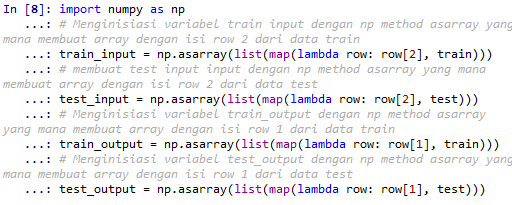
\includegraphics[width=4cm]{figures/1174077/7/praktek_4.PNG}
		\caption{Hasil Soal 4.}
	\end{figure}

	\item Jelaskan kode program pada blok \# In[5]. Jelaskan arti dari setiap baris kode yang dibuat(harus beda dengan teman sekelas) dan hasil luarannya dari komputer sendiri.
	\hfill\break
	\lstinputlisting[firstline=61, lastline=66]{src/1174077/7/1174077.py}
	\begin{figure}[H]
	\centering
		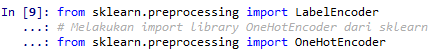
\includegraphics[width=4cm]{figures/1174077/7/praktek_5.PNG}
		\caption{Hasil Soal 5.}
	\end{figure}

	\item Jelaskan kode program pada blok \# In[6]. Jelaskan arti dari setiap baris kode yang dibuat(harus beda dengan teman sekelas) dan hasil luarannya dari komputer sendiri.
	\hfill\break
	\lstinputlisting[firstline=67, lastline=73]{src/1174077/7/1174077.py}
	\begin{figure}[H]
	\centering
		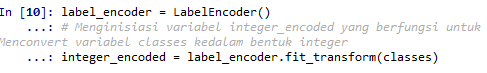
\includegraphics[width=4cm]{figures/1174077/7/praktek_6.PNG}
		\caption{Hasil Soal 6.}
	\end{figure}

	\item Jelaskan kode program pada blok \# In[7]. Jelaskan arti dari setiap baris kode yang dibuat(harus beda dengan teman sekelas) dan hasil luarannya dari komputer sendiri.
	\hfill\break
	\lstinputlisting[firstline=78, lastline=81]{src/1174077/7/1174077.py}
	\begin{figure}[H]
	\centering
		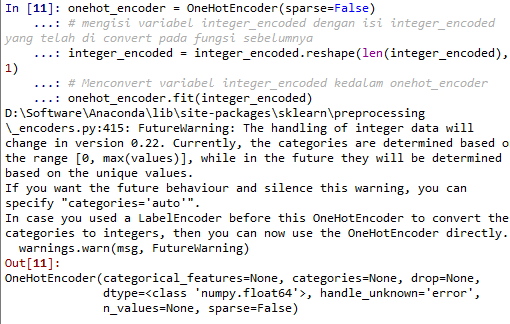
\includegraphics[width=4cm]{figures/1174077/7/praktek_7.PNG}
		\caption{Hasil Soal 7.}
	\end{figure}

	\item Jelaskan kode program pada blok \# In[8]. Jelaskan arti dari setiap baris kode yang dibuat(harus beda dengan teman sekelas) dan hasil luarannya dari komputer sendiri.
	\hfill\break
	\lstinputlisting[firstline=79, lastline=91]{src/1174077/7/1174077.py}
	\begin{figure}[H]
	\centering
		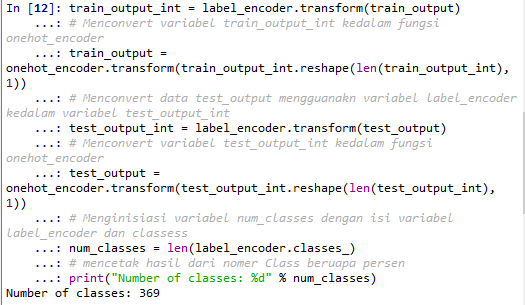
\includegraphics[width=4cm]{figures/1174077/7/praktek_8.PNG}
		\caption{Hasil Soal 8.}
	\end{figure}

	\item Jelaskan kode program pada blok \# In[9]. Jelaskan arti dari setiap baris kode yang dibuat(harus beda dengan teman sekelas) dan hasil luarannya dari komputer sendiri.
	\hfill\break
	\lstinputlisting[firstline=93, lastline=99]{src/1174077/7/1174077.py}
	\begin{figure}[H]
	\centering
		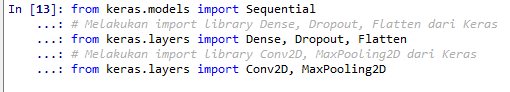
\includegraphics[width=4cm]{figures/1174077/7/praktek_9.PNG}
		\caption{Hasil Soal 9.}
	\end{figure}

	\item Jelaskan kode program pada blok \# In[10]. Jelaskan arti dari setiap baris kode yang dibuat(harus beda dengan teman sekelas) dan hasil luarannya dari komputer sendiri.
	\hfill\break
	\lstinputlisting[firstline=101, lastline=125]{src/1174077/7/1174077.py}
	\begin{figure}[H]
	\centering
		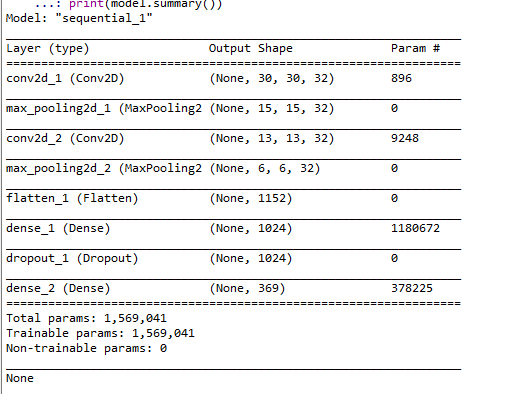
\includegraphics[width=4cm]{figures/1174077/7/praktek_10.PNG}
		\caption{Hasil Soal 10.}
	\end{figure}

	\item Jelaskan kode program pada blok \# In[11]. Jelaskan arti dari setiap baris kode yang dibuat(harus beda dengan teman sekelas) dan hasil luarannya dari komputer sendiri.
	\hfill\break
	\lstinputlisting[firstline=127, lastline=131]{src/1174077/7/1174077.py}
	\begin{figure}[H]
	\centering
		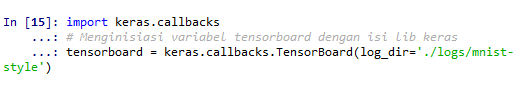
\includegraphics[width=4cm]{figures/1174077/7/praktek_11.PNG}
		\caption{Hasil Soal 11.}
    \end{figure}
    
    \item Jelaskan kode program pada blok \# In[12]. Jelaskan arti dari setiap baris kode yang dibuat(harus beda dengan teman sekelas) dan hasil luarannya dari komputer sendiri.
    \hfill\break
    \lstinputlisting[firstline=133, lastline=145]{src/1174077/7/1174077.py}
    \begin{figure}[H]
        \centering
            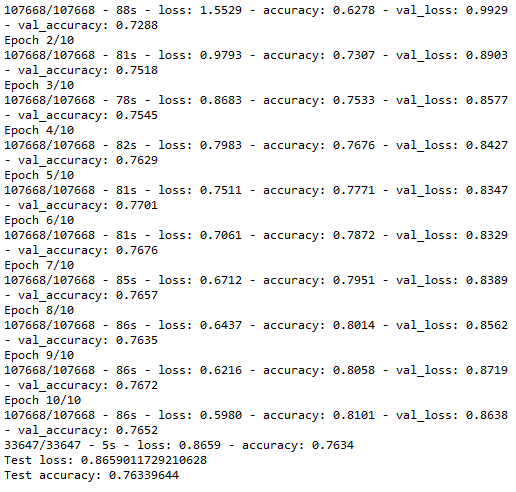
\includegraphics[width=4cm]{figures/1174077/7/praktek_12.PNG}
            \caption{Hasil Soal 12.}
        \end{figure}
        
    \item Jelaskan kode program pada blok \# In[13]. Jelaskan arti dari setiap baris kode yang dibuat(harus beda dengan teman sekelas) dan hasil luarannya dari komputer sendiri.
    \hfill\break
    \lstinputlisting[firstline=153, lastline=208]{src/1174077/7/1174077.py}
    \begin{figure}[H]
        \centering
            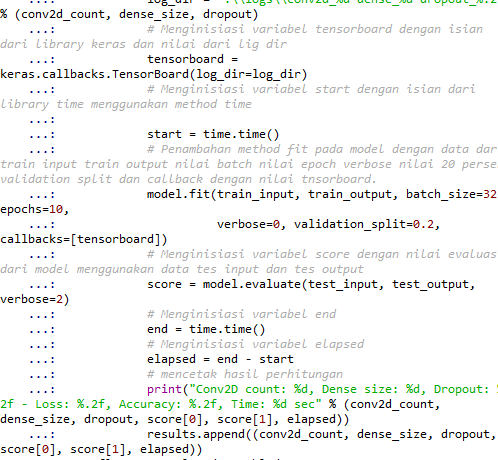
\includegraphics[width=4cm]{figures/1174077/7/praktek_13.PNG}
            \caption{Hasil Soal 13.}
        \end{figure}
        
    \item Jelaskan kode program pada blok \# In[14]. Jelaskan arti dari setiap baris kode yang dibuat(harus beda dengan teman sekelas) dan hasil luarannya dari komputer sendiri.
    \hfill\break
    \lstinputlisting[firstline=211, lastline=233]{src/1174077/7/1174077.py}
    \begin{figure}[H]
        \centering
            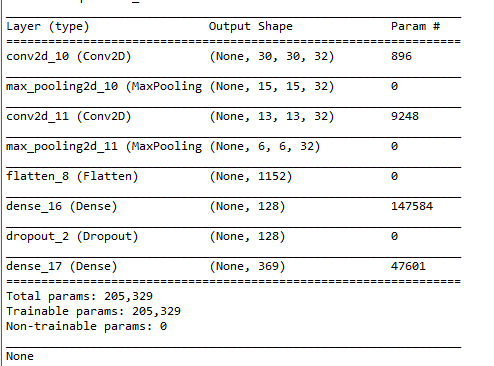
\includegraphics[width=4cm]{figures/1174077/7/praktek_14.PNG}
            \caption{Hasil Soal 14.}
        \end{figure}
        
    \item Jelaskan kode program pada blok \# In[15]. Jelaskan arti dari setiap baris kode yang dibuat(harus beda dengan teman sekelas) dan hasil luarannya dari komputer sendiri.
    \hfill\break
    \lstinputlisting[firstline=234, lastline=240]{src/1174077/7/1174077.py}
    \begin{figure}[H]
        \centering
            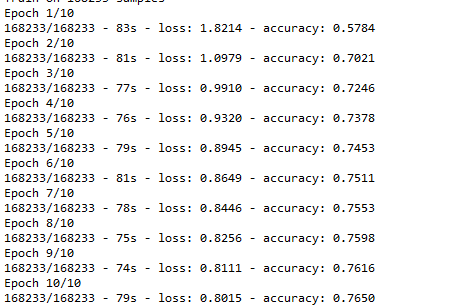
\includegraphics[width=4cm]{figures/1174077/7/praktek_15.PNG}
            \caption{Hasil Soal 15.}
        \end{figure}
        
    \item Jelaskan kode program pada blok \# In[16]. Jelaskan arti dari setiap baris kode yang dibuat(harus beda dengan teman sekelas) dan hasil luarannya dari komputer sendiri.
    \hfill\break
    \lstinputlisting[firstline=242, lastline=244]{src/1174077/7/1174077.py}
    \begin{figure}[H]
        \centering
            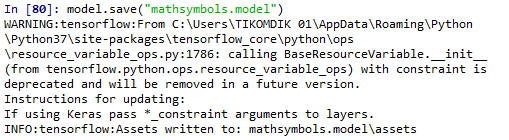
\includegraphics[width=4cm]{figures/1174077/7/praktek_16.PNG}
            \caption{Hasil Soal 16.}
        \end{figure}
        
    \item Jelaskan kode program pada blok \# In[17]. Jelaskan arti dari setiap baris kode yang dibuat(harus beda dengan teman sekelas) dan hasil luarannya dari komputer sendiri.
    \hfill\break
    \lstinputlisting[firstline=246, lastline=248]{src/1174077/7/1174077.py}
    \begin{figure}[H]
        \centering
            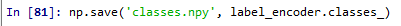
\includegraphics[width=4cm]{figures/1174077/7/praktek_17.PNG}
            \caption{Hasil Soal 17.}
        \end{figure}
        
    \item Jelaskan kode program pada blok \# In[18]. Jelaskan arti dari setiap baris kode yang dibuat(harus beda dengan teman sekelas) dan hasil luarannya dari komputer sendiri.
    \hfill\break
    \lstinputlisting[firstline=251, lastline=258]{src/1174077/7/1174077.py}
    \begin{figure}[H]
        \centering
            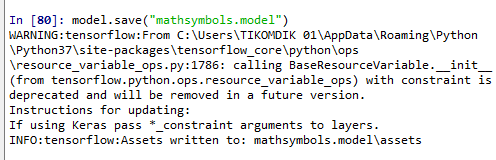
\includegraphics[width=4cm]{figures/1174077/7/praktek_18.PNG}
            \caption{Hasil Soal 18.}
        \end{figure}
        
    \item Jelaskan kode program pada blok \# In[19]. Jelaskan arti dari setiap baris kode yang dibuat(harus beda dengan teman sekelas) dan hasil luarannya dari komputer sendiri.
    \hfill\break
    \lstinputlisting[firstline=260, lastline=280]{src/1174077/7/1174077.py}
    \begin{figure}[H]
        \centering
            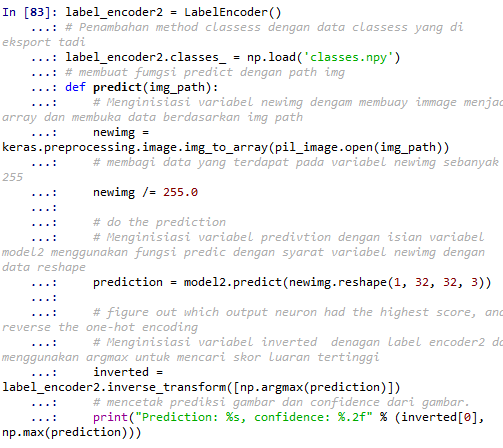
\includegraphics[width=4cm]{figures/1174077/7/praktek_19.PNG}
            \caption{Hasil Soal 19.}
        \end{figure}
        
    \item Jelaskan kode program pada blok \# In[20]. Jelaskan arti dari setiap baris kode yang dibuat(harus beda dengan teman sekelas) dan hasil luarannya dari komputer sendiri.
    \hfill\break
    \lstinputlisting[firstline=282, lastline=288]{src/1174077/7/1174077.py}
    \begin{figure}[H]
        \centering
            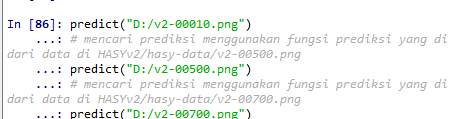
\includegraphics[width=4cm]{figures/1174077/7/praktek_20.PNG}
            \caption{Hasil Soal 20.}
        \end{figure}
        
\end{enumerate}

\subsection{Penanganan Error}
\begin{enumerate}
	\item ModuleNotFoundError: No module named 'keras'
	\begin{figure}[H]
		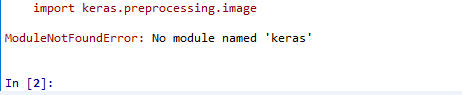
\includegraphics[width=4cm]{figures/1174077/7/error.PNG}
		\centering
		\caption{NameError}
	\end{figure}
	\item Tuliskan Kode Error dan Jenis Error
	\begin{itemize}
		\item ModuleNotFoundError
	\end{itemize}
	\item Cara Penangan Error
	\begin{itemize}
		\item ModuleNotFoundError
		\hfill\break
		Error terjadi karena belum dilakukan instalasi keras pada komputer. Sehingga library keras tidak dapat dipanggil. Untuk mengatasinya, lakukan instalasi library keras terlebih dahulu pada komputer.
	\end{itemize}
\end{enumerate}

\subsection{Bukti Tidak Plagiat}
\begin{figure}[H]
\centering
	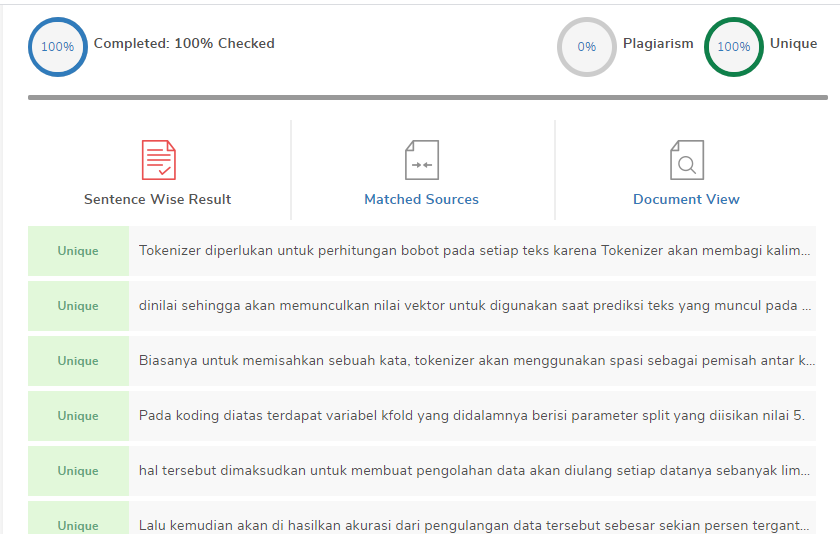
\includegraphics[width=4cm]{figures/1174077/7/plagiarisme.PNG}
	\caption{Bukti Tidak Melakukan Plagiat Chapter 7}
\end{figure}

